\documentclass[11pt]{amsart}
\usepackage[margin=1.15in]{geometry}
\usepackage[T1]{fontenc}
\usepackage{lmodern}
\usepackage{amssymb,amsmath,mathtools}
\usepackage{graphicx,float}
\usepackage[hidelinks]{hyperref}
\usepackage[expansion=false]{microtype}

\newtheorem{theorem}{Theorem}[section]
\newtheorem{proposition}[theorem]{Proposition}
\newtheorem{lemma}[theorem]{Lemma}
\newtheorem{corollary}[theorem]{Corollary}
\newtheorem{mainthm}{Theorem}
\renewcommand{\themainthm}{\Alph{mainthm}}
\theoremstyle{definition}
\newtheorem{definition}[theorem]{Definition}
\newtheorem{remark}[theorem]{Remark}

\newcommand{\CC}{\mathbb{C}}
\newcommand{\ZZ}{\mathbb{Z}}
\newcommand{\EE}{\mathbb{E}}
\newcommand{\PP}{\mathbb{P}}
\newcommand{\dd}{\,\mathrm{d}}
\newcommand{\Tr}{\operatorname{Tr}}
\newcommand{\rb}{\bar\rho}
\newcommand{\ket}[1]{\lvert #1\rangle}
\newcommand{\bra}[1]{\langle #1\rvert}

\setlength{\emergencystretch}{2.5em}
\hbadness=2000
\raggedbottom
\begin{document}

\title[Periodicity and Boltzmann brains]{Exact Periodicity Does Not Evade\\ the Boltzmann Brain Problem}

\author{Deep Bhattacharjee}
\address{Formerly, Electro-Gravitational Space Propulsion Laboratory (EGSPL), Bhubaneswar, Odisha 751030, India}
\address{Formerly, University of Calcutta (Heramba Chandra College), 23/49 Gariahat Road, Golpark, Kolkata 700029, West Bengal, India}
\email{d.bhattacharjee@erl-forschung.de}
\email{itsdeep@live.com}
\email{egspl@proton.me (GitHub-related contact; GitHub account creelie)}
\urladdr{https://orcid.org/0000-0003-0466-750X}

\begin{abstract}
Carroll, Diachenko and Dulani proposed that a finite quantum universe with commensurable energy levels evolves periodically, and that its low-entropy bounce then recurs far more often than the law $e^{-\Delta S}$ allows, so that ordinary observers outnumber Boltzmann brains. We prove that this is not so. Born-weighted rates do not depend on whether the spectrum is commensurable. For macrostates in general position, the minimal macrostate carries weight $(d+1)/(D+1)$, and for all but a small fraction of placements the period obeys $T\,\Delta E\gtrsim(D+1)/(d+1)$. The proposed range of periods is therefore empty unless the macrostates are fine-tuned or the dynamics explores no more entropy than a single Boltzmann brain.

\medskip\noindent\textbf{Keywords:} quantum recurrence; Boltzmann brains; diagonal ensemble.

\smallskip\noindent\textbf{MSC 2020:} 81P05 (primary); 82B03, 83F05.
\end{abstract}

\maketitle

\section{Introduction}\label{sec:intro}

If the universe is a pure state $\psi(t)$ evolving unitarily in a Hilbert space of finite dimension $D$, its evolution is recurrent \cite{BL57}. Recurrence brings the Boltzmann brain problem \cite{DKS02,AS04}. A system that spends most of its time near equilibrium makes downward entropy fluctuations of size $\Delta S$ with relative frequency of order $e^{-\Delta S}$. Small fluctuations then vastly outnumber the single large one that a Big Bang requires, and a typical observer is a fluctuation rather than the product of a low-entropy past.

Carroll, Diachenko and Dulani \cite{CDD26} propose a way out. Following \cite{Car23}, they take the shifted energies to be commensurable, $E_k-E_0=p_k\omega_*$ with $p_k\in\ZZ$. The evolution is then exactly periodic with period $T_*=2\pi/\omega_*$, and its orbit is a closed curve in the torus of phases rather than a dense winding. Coarse-graining is a decomposition $\CC^D=\bigoplus_a\mathcal H_a$ into macrostates of dimensions $d_a$ with projectors $\Pi_a$. The quantum Boltzmann entropy is
\begin{equation}\label{eq:SQB}
S_{\rm QB}(t)=\sum_a p_a(t)\log d_a,\qquad p_a(t)=\langle\psi(t)|\Pi_a|\psi(t)\rangle .
\end{equation}
Starting in the smallest macrostate, the authors argue that the bounce at $t=0$ ``can periodically repeat on a much shorter timescale than one would expect from $\exp(-\Delta S)$ statistics''. They support this with a simulation ($D=111$, macrostates of dimensions $1,10,100$ placed Haar-randomly relative to the energy basis, energies equal to random integers in $[1,1000]$ times $\omega_*$). Ordinary observers are counted once per period and Boltzmann brains at a fixed rate per unit time. This gives the criterion $T_*\le e^{10^{66}}$, and the authors conclude that a period in the range
\begin{equation}\label{eq:window}
10^{10}\,\mathrm{yr}\le T_*\le e^{10^{66}}
\end{equation}
``should be completely allowed''. Observers on different branches are to be weighted ``by the amplitude-squared of the branches that they are on, \dots\ so a standard expectation value in a single stochastic universe is what we want'' \cite[footnote~2]{CDD26}.

We show that the argument fails. Throughout, $H=\sum_{j=1}^{L}E_jP_j$ is the spectral decomposition of the Hamiltonian into distinct eigenvalues $E_1<\dots<E_L$ with multiplicities $m_j=\operatorname{rank}P_j$. The initial state is a unit vector $\psi_0$ in the range of a macrostate projector $\Pi$ of rank $d$. We write $q_j=\|P_j\psi_0\|^2$, $M=\#\{j:q_j>0\}$, $\Delta E^2=\sum_jq_jE_j^2-(\sum_jq_jE_j)^2$, and
\begin{equation}\label{eq:rhobar}
\rb=\sum_jP_j\ket{\psi_0}\bra{\psi_0}P_j,\qquad \bar p=\Tr(\rb\,\Pi).
\end{equation}
A \emph{period} of the evolution is any $T>0$ for which $\psi(T)$ is a multiple of $\psi_0$. Such a $T$ exists exactly when the populated gaps are commensurable, and then every populated gap lies in $(2\pi/T)\ZZ$.

\begin{mainthm}[Spectral invariance]\label{thm:A}
For every operator $A$ the long-time average of $\langle\psi(t)|A|\psi(t)\rangle$ equals $\Tr(\rb A)$. When the evolution has a period $T$, the average over any interval of length $T$ already equals $\Tr(\rb A)$. In particular, every Born-weighted rate of events depends on $H$ only through its spectral projections. Every commensurable $H$ with at least three distinct eigenvalues is a limit of incommensurable Hamiltonians with exactly the same Born-weighted rates.
\end{mainthm}

\begin{mainthm}[Weight of the minimal macrostate]\label{thm:B}
One has $\sum_jq_j^2\le\bar p\le\max_j\|P_j\Pi P_j\|$, and $\sum_j q_j^2\ge 1/M$. If the macrostate decomposition is placed Haar-randomly relative to the eigenspaces, with $\psi_0$ correspondingly random in $\mathcal H_1$, then
\begin{equation}\label{eq:haar}
\EE\,\bar p=\sum_{j=1}^L\frac{m_j(m_j+1)+(d-1)\,m_j(D-m_j)/(D-1)}{D(D+1)} .
\end{equation}
For a nondegenerate spectrum this equals $(d+1)/(D+1)$, and in general $\EE\,\bar p\le\sum_j(m_j/D)^2+d/(D+1)$.
\end{mainthm}

\begin{mainthm}[The period is not free]\label{thm:C}
Let $T$ be a period and suppose $\bar p\le 8/15$. Then
\[
T\,\Delta E\ \ge\ \frac{16\sqrt2}{15}\,\frac1{\bar p}\ >\ \frac{1.5}{\bar p}.
\]
Moreover, if $W$ is the spread of the populated energies, then $M\le 1+WT/2\pi$, so the von Neumann and R\'enyi-2 entropies of $\rb$ are at most $\log(1+WT/2\pi)$.
\end{mainthm}

Theorem~\ref{thm:A} removes the mechanism. The only role of commensurability in \cite{CDD26} is to make the bounce recur at full weight. Under the Born weighting that the authors prescribe, a full-weight bounce once per period produces exactly the same expected numbers of every kind of observer, per unit time, as the partial near-recurrences of a nearby incommensurable spectrum. Theorems~\ref{thm:B} and~\ref{thm:C} show that nothing replaces the mechanism. In the ensemble used in \cite{CDD26}, the minimal macrostate is occupied for the fraction $(d+1)/(D+1)$ of the time. That is the $e^{-\Delta S}$ law up to a factor at most $2$, and bounces can recur no faster than $\Delta E\,\bar p/1.5$. Corollary~\ref{cor:window} applies this to the range \eqref{eq:window}.

The facts behind Theorem~\ref{thm:A} go back to von Neumann's dephasing argument \cite{vN29} and underlie the modern treatment of equilibration \cite{Rei08,LPSW09}. The state $\rb$ is the diagonal ensemble, and its entropy is the diagonal entropy of \cite{Pol11}. What is new is their application to the proposal of \cite{CDD26}, the exact Haar formula \eqref{eq:haar}, and the period bound of Theorem~\ref{thm:C}.

\section{Dephasing and spectral invariance}\label{sec:A}

\begin{proof}[Proof of Theorem~\ref{thm:A}]
Since $\psi(t)=\sum_je^{-iE_jt}P_j\psi_0$,
\[
\langle\psi(t)|A|\psi(t)\rangle=\sum_{j,l}e^{i(E_j-E_l)t}\langle P_j\psi_0|A|P_l\psi_0\rangle .
\]
For $\nu\neq0$, $\frac1T\int_{t_0}^{t_0+T}e^{i\nu t}\dd t=e^{i\nu t_0}(e^{i\nu T}-1)/(i\nu T)$. This tends to $0$ as $T\to\infty$, and it vanishes identically when $\nu\in(2\pi/T)\ZZ\setminus\{0\}$. Every off-diagonal frequency $E_j-E_l$ with $q_j q_l>0$ is of this kind when $T$ is a period, and terms with $q_jq_l=0$ vanish. Only the diagonal $j=l$ survives, and it gives $\sum_j\langle P_j\psi_0|A|P_j\psi_0\rangle=\Tr(\rb A)$.

A Born-weighted count of events of a given kind up to time $\tau$ has the form $N_O(\tau)=\int_0^\tau\langle\psi(t)|O|\psi(t)\rangle\dd t$ for a positive operator $O$. Its rate $\lim N_O(\tau)/\tau=\Tr(\rb O)$ depends on the projections $P_j$ but not on the numbers $E_j$. Given a commensurable $H$, put $H_\varepsilon=\sum_j(E_j+\varepsilon\eta_j)P_j$ with $\eta_j=\sqrt{\pi_j}$ for distinct primes $\pi_j$. For small $\varepsilon>0$ the order of the eigenvalues is unchanged. If $L\ge3$, the ratio of the gaps $E_2-E_1+\varepsilon(\eta_2-\eta_1)$ and $E_3-E_1+\varepsilon(\eta_3-\eta_1)$ is a nonconstant M\"obius function of $\varepsilon$, because $(\eta_2-\eta_1)/(\eta_3-\eta_1)$ is irrational by the linear independence of square roots of distinct primes over $\mathbb Q$; it is therefore irrational for all but countably many $\varepsilon$. So $H_\varepsilon$ is incommensurable, $H_\varepsilon\to H$, and $H_\varepsilon$ has the same projections and hence the same rates.
\end{proof}

\begin{remark}\label{rem:count}
The criterion behind \eqref{eq:window} compares $N_{\rm OO}$ ordinary observers per period with $N_{\rm BB}=\Gamma_{\rm BB}T_*H_*^{-3}$ Boltzmann brains per period. Under Born weighting the first number is a rate $N_{\rm OO}/T_*=\Tr(\rb\,O_{\rm OO})$ and the second is $\Tr(\rb\,O_{\rm BB})$. By Theorem~\ref{thm:A} their ratio is the same for $H$ and for every $H_\varepsilon$, whose evolution has no period at all. The ratio therefore cannot be controlled by the length of the period. What it does depend on is the diagonal ensemble, and Theorems~\ref{thm:B} and~\ref{thm:C} show what the diagonal ensemble allows.
\end{remark}

\section{The weight of the minimal macrostate}\label{sec:B}

\begin{proof}[Proof of the deterministic part of Theorem~\ref{thm:B}]
By \eqref{eq:rhobar}, $\bar p=\sum_j\|\Pi P_j\psi_0\|^2$. Since $\Pi\psi_0=\psi_0$, the Cauchy--Schwarz inequality gives $\|\Pi P_j\psi_0\|\ge|\langle\psi_0|\Pi P_j\psi_0\rangle|=|\langle\psi_0|P_j\psi_0\rangle|=q_j$. Hence $\bar p\ge\sum_jq_j^2\ge(\sum_jq_j)^2/M=1/M$. For the upper bound, $\|\Pi P_j\psi_0\|^2=\langle P_j\psi_0|P_j\Pi P_j|P_j\psi_0\rangle\le\|P_j\Pi P_j\|\,q_j$, and $\sum_jq_j=1$.
\end{proof}

The lower bound $\sum_jq_j^2=\Tr(\rb^{\,2})$ is the time-averaged return probability. The upper bound says that the minimal macrostate can be occupied much more often than its share of Hilbert space only if it overlaps some eigenspace of $H$ much more than its share. That is a statement about the position of $\mathcal H_1$ relative to the eigenspaces, not about the eigenvalues.

For the random part we use the model of \cite{CDD26}. Fix the eigenspaces, fix an orthonormal basis $e_1,\dots,e_D$ and a partition of $\{1,\dots,D\}$ into blocks $B_a$ of sizes $d_a$ with $1\in B_1$. Let $U$ be Haar-distributed on $\mathrm U(D)$, and put $\mathcal H_a=U\,\mathrm{span}\{e_i:i\in B_a\}$ and $\psi_0=Ue_1$. Because the Haar measure is invariant under unitaries of $\mathcal H_1$, this gives the same law as an arbitrary rule for choosing $\psi_0$ in $\mathcal H_1$ that is unitarily covariant.

\begin{lemma}\label{lem:beta}
Let $u$ be uniform on the unit sphere of $\CC^D$ and $P$ a projector of rank $m$. Then $q=\langle u|P|u\rangle$ satisfies $\EE q=m/D$ and $\EE q^2=m(m+1)/(D(D+1))$. If $v$ is uniform on the unit sphere of $u^\perp$, then $\EE\,|\langle v|P|u\rangle|^2=m(D-m)/(D(D+1)(D-1))$.
\end{lemma}

\begin{proof}
Write $u=g/\|g\|$ with $g$ a standard complex Gaussian vector, and take $P$ diagonal, which is allowed by unitary invariance. The variables $|g_i|^2$ are independent and exponential with mean one. So $q=X/(X+Y)$ with independent $X\sim\Gamma(m)$ and $Y\sim\Gamma(D-m)$, that is, $q$ has the Beta$(m,D-m)$ law, whose first two moments are those stated. Given $u$, the vector $v$ is invariant in law under unitaries fixing $u$, so $\EE[\ket v\bra v\mid u]=(I-\ket u\bra u)/(D-1)$. Hence
\[
\EE\big[|\langle v|Pu\rangle|^2\mid u\big]=\frac{\|Pu\|^2-|\langle u|Pu\rangle|^2}{D-1}=\frac{q-q^2}{D-1},
\]
and taking expectations gives $\big(m/D-m(m+1)/(D(D+1))\big)/(D-1)=m(D-m)/(D(D+1)(D-1))$.
\end{proof}

\begin{proof}[Proof of \eqref{eq:haar}]
Since $\Pi_1=\sum_{i\in B_1}\ket{Ue_i}\bra{Ue_i}$,
\[
\bar p=\sum_j\sum_{i\in B_1}|\langle Ue_i|P_j|Ue_1\rangle|^2 .
\]
The vector $u=Ue_1$ is uniform on the sphere, and for $i\neq1$ the vector $Ue_i$ is uniform on the sphere of $u^\perp$. Lemma~\ref{lem:beta} gives $m_j(m_j+1)/(D(D+1))$ for $i=1$ and $m_j(D-m_j)/(D(D+1)(D-1))$ for each of the $d-1$ other indices. Summing over $j$ gives \eqref{eq:haar}. If every $m_j=1$, then $L=D$ and each summand is $(d+1)/(D(D+1))$. In general $(D-m_j)/(D-1)\le1$ and $\sum_jm_j=D$, so $\EE\bar p\le(\sum_jm_j^2+dD)/(D(D+1))\le\sum_j(m_j/D)^2+d/(D+1)$.
\end{proof}

For the other macrostates the same computation gives $\EE\,\Tr(\rb\,\Pi_a)=d_a/(D+1)$ for $a\neq1$ in the nondegenerate case, and the weights sum to one. So in the ensemble of \cite{CDD26} the diagonal ensemble gives every macrostate its share of Hilbert space. The macrostate holding the initial state gets one extra unit, $(d_1+1)$ in place of $d_1$, and no more.

\begin{remark}[The simulation of \cite{CDD26}]\label{rem:sim}
There $d_1=1$ and the $D=111$ energies are independent uniform integers in $[1,1000]$, so ties occur. With $d=1$, formula \eqref{eq:haar} reads $\EE\bar p=(D+\sum_jm_j^2)/(D(D+1))$. Since $\EE\sum_jm_j^2=\sum_{k,k'}\PP(E_k=E_{k'})=D+D(D-1)/1000$, we get $\EE\bar p=234.21/12432\approx1/53$. This is about twice $d_1/D=1/111$, as Theorem~\ref{thm:B} predicts. The weight is not concentrated at the bounce. Figure~\ref{fig:weight} shows one realisation of this set-up, where the window $|t|\le3/\Delta E$ around the bounce carries $6\%$ of the time-averaged weight of $\mathcal H_1$. The remaining $94\%$ comes from the small fluctuations of the equilibrium phase. The figure is an illustration only and is not used in any proof.
\end{remark}

\begin{figure}[H]
\centering
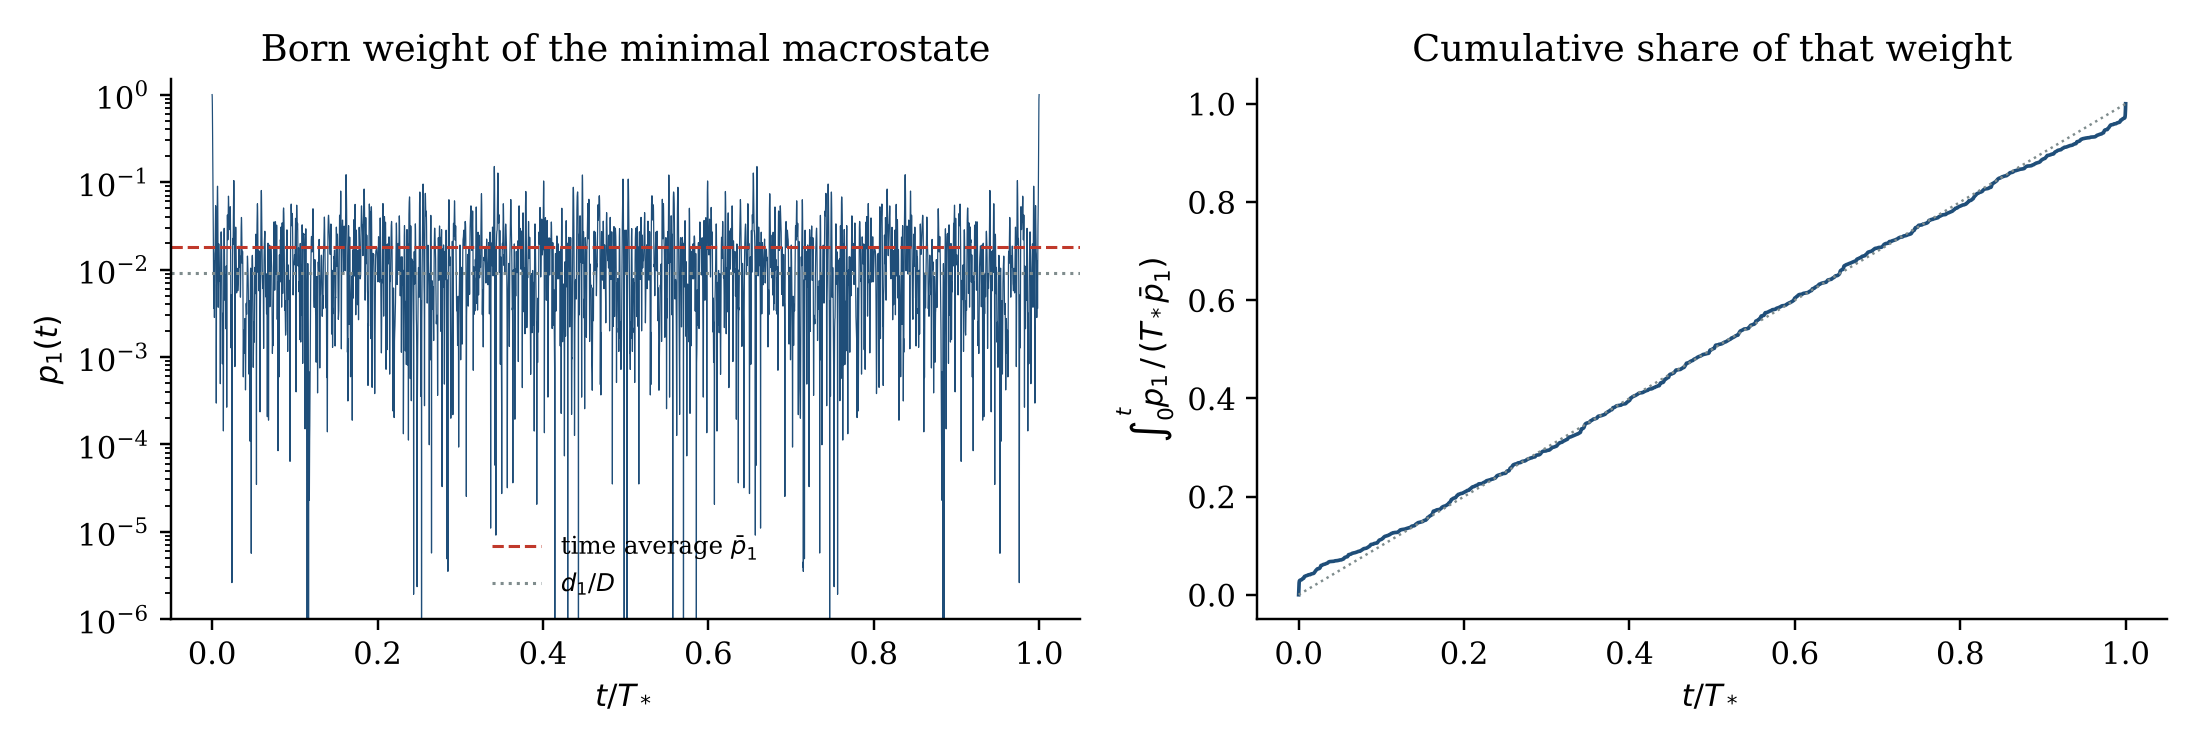
\includegraphics[width=\textwidth]{fig_weight.png}
\caption{One realisation of the set-up of \cite{CDD26}: $D=111$, $d_a=1,10,100$, energies uniform integers in $[1,1000]$ (period $T_*=2\pi/\omega_*$). Left: $p_1(t)$ on a logarithmic scale, with its time average $\bar p_1\approx0.018$ and the share $d_1/D$. Right: cumulative fraction of $\int p_1$ over one period. The bounces at $t=0$ and $t=T_*$ add a visible but small step to an otherwise uniform growth.}
\label{fig:weight}
\end{figure}

\section{The period bound}\label{sec:C}

\begin{lemma}\label{lem:return}
For all real $t$, $|\langle\psi_0|\psi(t)\rangle|\ge1-\tfrac12\Delta E^2t^2$, and therefore $p(t)=\|\Pi\psi(t)\|^2\ge\big(1-\tfrac12\Delta E^2t^2\big)^2$ whenever $|t|\le\sqrt2/\Delta E$.
\end{lemma}

\begin{proof}
Let $\bar E=\sum_jq_jE_j$. Then $|\langle\psi_0|\psi(t)\rangle|=|\sum_jq_je^{-i(E_j-\bar E)t}|\ge\sum_jq_j\cos((E_j-\bar E)t)$. Using $\cos x\ge1-x^2/2$ bounds this below by $1-\tfrac12\Delta E^2t^2$. Since $\Pi\psi_0=\psi_0$, we have $|\langle\psi_0|\psi(t)\rangle|=|\langle\psi_0|\Pi\psi(t)\rangle|\le\|\Pi\psi(t)\|$.
\end{proof}

This is an elementary form of the Mandelstam--Tamm speed limit. Its only use here is to show that a bounce lasts for a time of order $1/\Delta E$.

\begin{proof}[Proof of Theorem~\ref{thm:C}]
By Theorem~\ref{thm:A}, $\bar p=\frac1T\int_{-T/2}^{T/2}p(t)\dd t$. Put $s=T\Delta E$ and $g(x)=(1-x^2/2)^2$ for $|x|\le\sqrt2$.

If $s<2\sqrt2$, Lemma~\ref{lem:return} applies on the whole interval and gives $\bar p\ge\frac1s\int_{-s/2}^{s/2}g(x)\dd x$. The right side decreases in $s$, since $g$ decreases in $|x|$, and at $s=2\sqrt2$ it equals $\frac1{2\sqrt2}\int_{-\sqrt2}^{\sqrt2}g=\frac{1}{2\sqrt2}\cdot\frac{16\sqrt2}{15}=\frac8{15}$. This would force $\bar p>8/15$, so the hypothesis gives $s\ge2\sqrt2$. In that case we integrate only over $|t|\le\sqrt2/\Delta E$ and use $p\ge0$ elsewhere:
\[
\bar p\ \ge\ \frac1{T\Delta E}\int_{-\sqrt2}^{\sqrt2}\Big(1-\frac{x^2}2\Big)^2\dd x=\frac{16\sqrt2}{15}\,\frac1{T\Delta E},
\]
which is the first claim.

For the second claim, every populated gap $E_j-E_l$ lies in $(2\pi/T)\ZZ\cap[-W,W]$. So the populated energies are distinct points of an arithmetic progression of step $2\pi/T$ in an interval of length $W$, and there are at most $1+WT/2\pi$ of them. The operator $\rb$ has the orthogonal eigenvectors $P_j\psi_0$ with eigenvalues $q_j$. It therefore has rank $M$, and both its von Neumann entropy and its R\'enyi-2 entropy $-\log\sum_jq_j^2$ are at most $\log M$.
\end{proof}

Theorem~\ref{thm:C} is a rigorous version of the statement that bounces recur at most at the rate their Born weight allows. In the nondegenerate case with macrostates in general position, Theorem~\ref{thm:B} and Markov's inequality show that, for every $\delta\in(0,1)$, with probability at least $1-\delta$ we have $\bar p\le(d+1)/(\delta(D+1))$. On that event, simultaneously for \emph{every} choice of distinct eigenvalues with these eigenvectors that makes the evolution periodic,
\begin{equation}\label{eq:Tlower}
T\,\Delta E\ \ge\ 1.5\,\delta\,\frac{D+1}{d+1}\qquad\text{provided }\frac{d+1}{\delta(D+1)}\le\frac8{15}.
\end{equation}
The period thus grows like $e^{\Delta S}$ with $\Delta S=\log(D/d)$, contrary to the statement in \cite{CDD26} that $T_*$ has no dependence on the size of Hilbert space. This holds even though the evolution is exactly periodic. The authors' heuristic for the time to enter a macrostate, $e^{c(D-d)}/\delta E$, also overstates the scale. The correct Born-weighted scale is $e^{\Delta S}/\Delta E$, exponential in the entropy rather than in the dimension.

\section{Consequences for the proposed range of periods}\label{sec:window}

\begin{corollary}\label{cor:window}
Suppose a periodic finite quantum universe has period $T\le e^{10^{66}}$, with its populated energy spread $W$ and energy uncertainty $\Delta E$ at most $e^{O(1)}$ in Planck units. Suppose the initial state lies in a macrostate of dimension $d$, and the dimension $D$ is so large that $d/D\le e^{-10^{100}}$. Then:
\begin{enumerate}
\item the diagonal ensemble has von Neumann entropy at most $10^{66}+O(1)$;
\item $\bar p\ge e^{-10^{66}-O(1)}$, so for Haar-random macrostates the bound $\EE\bar p\le\sum_j(m_j/D)^2+d/(D+1)$ forces either $\sum_j(m_j/D)^2\ge\delta\,e^{-10^{66}-O(1)}$ or an event of probability less than $\delta$.
\end{enumerate}
\end{corollary}

\begin{proof}
Part (1) is the second half of Theorem~\ref{thm:C}, since $\log(1+WT/2\pi)\le10^{66}+O(1)$. For part (2), Theorem~\ref{thm:C} gives $\bar p\ge 1.5/(T\Delta E)\ge e^{-10^{66}-O(1)}$ when $\bar p\le8/15$, and trivially otherwise. By Markov's inequality, $\PP(\bar p\ge x)\le(\sum_j(m_j/D)^2+d/(D+1))/x$. Taking $x=e^{-10^{66}-O(1)}$ and using $d/(D+1)\le e^{-10^{100}}$ gives the dichotomy.
\end{proof}

The range \eqref{eq:window} is therefore reachable in only two ways, and commensurability plays no part in either.

The first is fine-tuning. The low-entropy macrostate must sit relative to the energy eigenspaces in a position whose Haar probability is double-exponentially small. In the de Sitter setting of \cite{CDD26}, with $D\sim e^{10^{122}}$, that probability is of order $e^{10^{66}-10^{122}}$.

The second is a spectrum concentrated on at most about $e^{10^{66}}$ effective levels, which is the degeneracy the authors invoke. By part (1), the state of the universe then explores a subspace of dimension at most about $e^{10^{66}}$, the dimension equivalent of the entropy $S_{\rm BB}\approx10^{66}$ of one Boltzmann brain used in \cite{CDD26}. Its equilibrium carries at most that much diagonal entropy, far from the $10^{122}$ of the de Sitter phase that the scenario identifies with equilibrium. The Boltzmann brain rate $\Gamma_{\rm BB}\sim e^{-M_{\rm BB}/T_{\rm dS}}$ that enters the criterion presupposes thermal fluctuations of a de Sitter patch with entropy $10^{122}$. A dynamics confined to a subspace of dimension $e^{10^{66}}$ does not supply that estimate.

Either way, the ratio of ordinary observers to fluctuations is fixed by the diagonal ensemble (Theorem~\ref{thm:A}). It is the same as for a nearby incommensurable universe with no recurrences at all.

\begin{remark}[What is correct in \cite{CDD26}]
The exact periodicity for commensurable gaps, the non-ergodicity of the orbit on the torus of phases, and the criterion for the symmetry $S_{\rm QB}(t)=S_{\rm QB}(-t)$ (reality of the Fourier coefficients of each $p_a$) are all correct. The discretisation of \cite{Car23} is also correct. With $N=\mathrm{lcm}(p_k)$ and $\gcd(p_k)=1$, the minimal period in steps is $\mathrm{lcm}_k(N/p_k)=N/\gcd_k(p_k)=N$. The error lies in the inference from periodicity to the suppression of Boltzmann fluctuations.
\end{remark}

The diagonal-ensemble viewpoint used here sits beside the author's earlier work on operator-theoretic and geometric structures \cite{Bha22a,Bha22b,BSN26}.

\section*{Declarations}

\noindent\textbf{Data availability.} No data were generated or analysed. All results are proved in the text. The \LaTeX\ source and the script that draws Figure~\ref{fig:weight}, which is not used in any proof, are archived at \url{https://doi.org/10.5281/zenodo.ZENODOID}.

\smallskip\noindent\textbf{Funding.} This research received no external funding.

\smallskip\noindent\textbf{Conflict of interest.} The author declares no conflict of interest.

\smallskip\noindent\textbf{Acknowledgements.} The periodic quantum cosmology examined here, its quantum Boltzmann entropy and its simulation are due to S.~M.~Carroll, N.~Diachenko and S.~Dulani. The dephasing argument is von Neumann's, and the diagonal entropy is Polkovnikov's.

\begin{thebibliography}{99}

\bibitem{AS04} A.~Albrecht and L.~Sorbo, Can the universe afford inflation?, \emph{Phys. Rev. D} \textbf{70} (2004), 063528. doi:10.1103/PhysRevD.70.063528.

\bibitem{Bha22a} D.~Bhattacharjee, Non-commutativity over canonical suspension $\eta$ for genus $g\ge1$ in hypercomplex structures for potential $\rho\phi$, \emph{Asian Res. J. Math.} \textbf{18} (2022), no.~11, 332--341. doi:10.9734/arjom/2022/v18i11607.

\bibitem{Bha22b} D.~Bhattacharjee, Establishing equivariant class $[O]$ for hyperbolic groups, \emph{Asian Res. J. Math.} \textbf{18} (2022), no.~11, 362--369. doi:10.9734/arjom/2022/v18i11615.

\bibitem{BSN26} D.~Bhattacharjee, S.~Singha Roy and P.~Nandi, Hodge--toric geometry beyond CY20, \emph{Int. J. Prof. Stud.} \textbf{21} (2026), no.~1. doi:10.37648/ijps.v21i01.019.

\bibitem{BL57} P.~Bocchieri and A.~Loinger, Quantum recurrence theorem, \emph{Phys. Rev.} \textbf{107} (1957), 337--338. doi:10.1103/PhysRev.107.337.

\bibitem{Car23} S.~M.~Carroll, Completely discretized, finite quantum mechanics, \emph{Found. Phys.} \textbf{53} (2023), 90. doi:10.1007/s10701-023-00726-6.

\bibitem{CDD26} S.~M.~Carroll, N.~Diachenko and S.~Dulani, Toward a phenomenologically acceptable quantum cyclic universe, preprint (2026), arXiv:2605.30405.

\bibitem{DKS02} L.~Dyson, M.~Kleban and L.~Susskind, Disturbing implications of a cosmological constant, \emph{J. High Energy Phys.} \textbf{2002} (2002), no.~10, 011. doi:10.1088/1126-6708/2002/10/011.

\bibitem{LPSW09} N.~Linden, S.~Popescu, A.~J.~Short and A.~Winter, Quantum mechanical evolution towards thermal equilibrium, \emph{Phys. Rev. E} \textbf{79} (2009), 061103. doi:10.1103/PhysRevE.79.061103.

\bibitem{Pol11} A.~Polkovnikov, Microscopic diagonal entropy and its connection to basic thermodynamic relations, \emph{Ann. Physics} \textbf{326} (2011), 486--499. doi:10.1016/j.aop.2010.08.004.

\bibitem{Rei08} P.~Reimann, Foundation of statistical mechanics under experimentally realistic conditions, \emph{Phys. Rev. Lett.} \textbf{101} (2008), 190403. doi:10.1103/PhysRevLett.101.190403.

\bibitem{vN29} J.~von Neumann, Beweis des Ergodensatzes und des $H$-Theorems in der neuen Mechanik, \emph{Z. Phys.} \textbf{57} (1929), 30--70. doi:10.1007/BF01339852.

\end{thebibliography}

\end{document}
